\chapter{Contexte du projet, problématique et méthodologie}

\section{Introduction}

Ce premier chapitre pose les fondations du projet de fin d'études. Il commence par présenter l'organisme d'accueil, \TT{}, et l'équipe au sein de laquelle le stage s'est déroulé, afin de situer le projet dans son contexte organisationnel et stratégique. Le cadrage de la demande est ensuite explicité, depuis le contexte technique général de la sécurité IoT jusqu'à la formulation précise de la problématique à laquelle le projet entend répondre. La dernière section décrit la méthodologie agile retenue, la planification temporelle (sprints, diagramme de Gantt) ainsi que les rôles et artefacts associés. Ce chapitre fournit ainsi le cadre nécessaire à la lecture des chapitres techniques qui suivent.

\section{Présentation de l'organisme d'accueil}

\subsection{Tunisie Telecom}

\TT{}, fondée en 1995 et privatisée partiellement en 2006, est l'opérateur historique de télécommunications en Tunisie. Avec plus de 7~millions d'abonnés fixes et mobiles, elle fournit des services de téléphonie, d'accès Internet haut débit (ADSL, fibre optique) et de solutions entreprise. \TT{} dispose d'une infrastructure réseau couvrant l'ensemble du territoire tunisien, incluant :

\begin{itemize}
  \item Un réseau cœur IP/MPLS interconnectant les différentes régions.
  \item Des data centers hébergeant les services cloud et d'hébergement.
  \item Une plate-forme IoT en cours de déploiement pour les projets Smart City et industrie~4.0.
\end{itemize}

L'opérateur est engagé dans une stratégie de transformation numérique qui place la sécurité des nouvelles infrastructures (cloud, IoT, 5G) au cœur de ses priorités opérationnelles.

\subsection{Service d'accueil et contexte du stage}

Le stage s'est déroulé au sein de l'équipe \textbf{Sécurité des Réseaux} de \TT{}, sous la supervision de \textbf{M.~Moez KHLIFI}. Cette équipe est en charge de la surveillance, de l'audit et du durcissement des infrastructures télécom de l'opérateur (réseaux cœur, data centers, services managés). Elle intervient à la fois en avant-vente (architecture sécurisée) et en exploitation (réponse aux incidents, conformité).

Le projet de fin d'études s'inscrit pleinement dans la stratégie de \TT{} visant à évaluer les solutions de sécurité adaptées aux déploiements IoT à grande échelle, en anticipation du déploiement commercial d'une plate-forme IoT publique. Il vise à produire un prototype de référence et un retour d'expérience utilisable par les architectes sécurité de l'opérateur.

\section{Cadrage de la demande}

\subsection{Contexte technique et motivations}

L'IoT présente des caractéristiques propres qui rendent sa sécurisation particulièrement délicate. Les dispositifs disposent souvent de ressources calculatoires limitées, leurs mises à jour de sécurité sont rares, et les protocoles de communication applicatifs (MQTT, CoAP) ont été conçus à l'origine sans mécanismes de sécurité obligatoires. Ces facteurs font des écosystèmes IoT des cibles privilégiées pour les attaquants, qui peuvent y déployer des \textit{botnets} (ex. Mirai), des attaques par déni de service (\ac{DoS}), des interceptions \textit{Man-in-the-Middle} ou encore des injections de données malveillantes.

Pour un opérateur télécom comme \TT{}, héberger ou transporter du trafic IoT non sécurisé représente un risque opérationnel et réputationnel majeur. La protection doit s'opérer simultanément sur plusieurs plans : authentification cryptographique des dispositifs, chiffrement des communications, détection d'intrusions réseau, corrélation centralisée des événements et détection comportementale par apprentissage automatique.

\subsection{Problématique}

La problématique centrale du projet peut se formuler ainsi :

\begin{tcolorbox}[colback=blue!5, colframe=blue!50!black, title=Problématique]
\textit{Comment sécuriser de bout en bout les flux de communication d'un écosystème IoT simulé, depuis l'authentification des dispositifs jusqu'à la détection automatisée des comportements anormaux, tout en maintenant des performances acceptables pour les applications temps-réel ?}
\end{tcolorbox}

Cette problématique se décompose en quatre sous-questions directrices :

\begin{enumerate}
  \item Comment établir une chaîne de confiance cryptographique pour des milliers de dispositifs IoT hétérogènes ?
  \item Comment configurer le protocole MQTT pour exiger une authentification mutuelle TLS (mTLS) sans dégrader significativement les performances ?
  \item Comment détecter en temps réel les attaques réseau et les comportements anormaux dans un flux MQTT chiffré ?
  \item Dans quelle mesure les approches de Machine Learning non supervisé sont-elles viables pour la détection d'anomalies dans des contextes IoT réels ?
\end{enumerate}

Pour répondre à ces questions, sept objectifs opérationnels ont été définis : déploiement d'une PKI dynamique (O1), configuration d'un broker mTLS strict (O2), simulation d'une flotte IoT réaliste (O3), analyse réseau IDS (O4), agrégation SIEM (O5), détection ML (O6) et évaluation des performances TLS (O7). Ces objectifs sont repris en synthèse dans la conclusion générale.

\section{Méthodologie de travail et planification}

\subsection{Méthodologie Scrum}

Pour mener à bien ce projet, nous avons adopté la méthodologie \textbf{Scrum}, un cadre de travail agile itératif et incrémental. Ce choix est motivé par :

\begin{itemize}
  \item La nature exploratoire du projet, nécessitant des ajustements fréquents de l'architecture.
  \item La nécessité de livrer des incréments fonctionnels à chaque itération pour validation par l'encadrant.
  \item La durée limitée du stage (environ 4~mois), imposant une gestion rigoureuse du temps et des priorités.
\end{itemize}

Scrum repose sur trois piliers fondamentaux : la \textbf{transparence}, l'\textbf{inspection} et l'\textbf{adaptation}. Dans le cadre de ce PFE, ces principes se sont traduits par un journal de bord quotidien (\texttt{JOURNAL.md}), des points d'avancement hebdomadaires avec l'encadrante universitaire et bimensuels avec l'encadrant entreprise, ainsi qu'un Product Backlog réajusté à chaque fin de sprint.

\begin{table}[H]
\centering
\caption{Répartition des rôles Scrum dans le projet}
\label{tab:roles_scrum}
\begin{tabular}{llp{6.5cm}}
\toprule
\textbf{Rôle} & \textbf{Personne} & \textbf{Responsabilité} \\
\midrule
Product Owner & M. Moez KHLIFI & Définition des besoins, priorisation du backlog, validation des livrables \\
Scrum Master & Mme. ELLOUZE NOURHENE & Suivi de l'avancement, levée des blocages, revue académique \\
Équipe Dev & Amine GHANNOUCHI & Conception, implémentation, tests, documentation \\
\bottomrule
\end{tabular}
\end{table}

\subsection{Product Backlog et planification des sprints}

Le Product Backlog initial a été établi lors du Sprint~0 (cadrage) et affiné itérativement. Le tableau~\ref{tab:product_backlog} présente les principales \textit{user stories} retenues.

\begin{longtable}{clp{7.2cm}c}
\caption{Product Backlog du projet}\label{tab:product_backlog}\\
\toprule
\textbf{ID} & \textbf{Priorité} & \textbf{Description} & \textbf{Sprint} \\
\midrule
\endfirsthead
\toprule
\textbf{ID} & \textbf{Priorité} & \textbf{Description} & \textbf{Sprint} \\
\midrule
\endhead
US-01 & Haute & Installer et configurer GNS3 avec VMware & 1 \\
US-02 & Haute & Créer la topologie réseau avec VLANs & 1 \\
US-03 & Haute & Déployer pfSense et MikroTik CHR & 1 \\
US-04 & Haute & Valider la connectivité inter-VLAN & 1 \\
US-05 & Haute & Déployer Vault et activer le moteur PKI & 2 \\
US-06 & Haute & Créer la hiérarchie CA racine + intermédiaire & 2 \\
US-07 & Haute & Configurer Mosquitto en TLS~1.3/mTLS & 2 \\
US-08 & Haute & Automatiser l'émission des certificats & 2 \\
US-09 & Moyenne & Développer le simulateur de flotte IoT & 3 \\
US-10 & Moyenne & Injecter le dataset CSV (76\,000 événements) & 3 \\
US-11 & Moyenne & Déployer Suricata avec règles MQTT & 4 \\
US-12 & Moyenne & Déployer Wazuh OVA et configurer l'ingestion & 4 \\
US-13 & Moyenne & Développer le pipeline ML (IF + RF) & 4 \\
US-14 & Basse & Réaliser les tests de performance TLS & 4 \\
US-15 & Basse & Rédiger le rapport et préparer la soutenance & 5 \\
\bottomrule
\end{longtable}

Le projet est organisé en \textbf{six sprints} d'une durée de deux à trois semaines chacun :

\begin{description}
  \item[Sprint 0 -- Cadrage (2~sem.)] Analyse des besoins, étude bibliographique, choix technologiques, validation du cahier des charges.
  \item[Sprint 1 -- Infrastructure réseau (3~sem.)] Topologie GNS3, VLANs, déploiement pfSense et MikroTik CHR, tests de connectivité.
  \item[Sprint 2 -- PKI et broker MQTT (3~sem.)] Vault, CA racine + intermédiaire, Mosquitto TLS~1.3/mTLS, émission des 50 certificats.
  \item[Sprint 3 -- Simulation de la flotte (2~sem.)] Développement du simulateur Python multi-thread, injection des 76\,000 messages.
  \item[Sprint 4 -- Détection et analyse (3~sem.)] Suricata, Wazuh OVA, règles de corrélation, pipeline ML, tests de performance.
  \item[Sprint 5 -- Synthèse et documentation (2~sem.)] Rédaction du rapport, diagrammes UML, préparation de la soutenance.
\end{description}

\subsection{Diagramme de Gantt}

Le diagramme de Gantt de la figure~\ref{fig:gantt} présente l'ordonnancement temporel détaillé des tâches sur l'ensemble des six sprints, ainsi que les jalons clés du projet (validation du cahier des charges, PKI opérationnelle, détection ML validée, soutenance).

\begin{figure}[H]
  \centering
  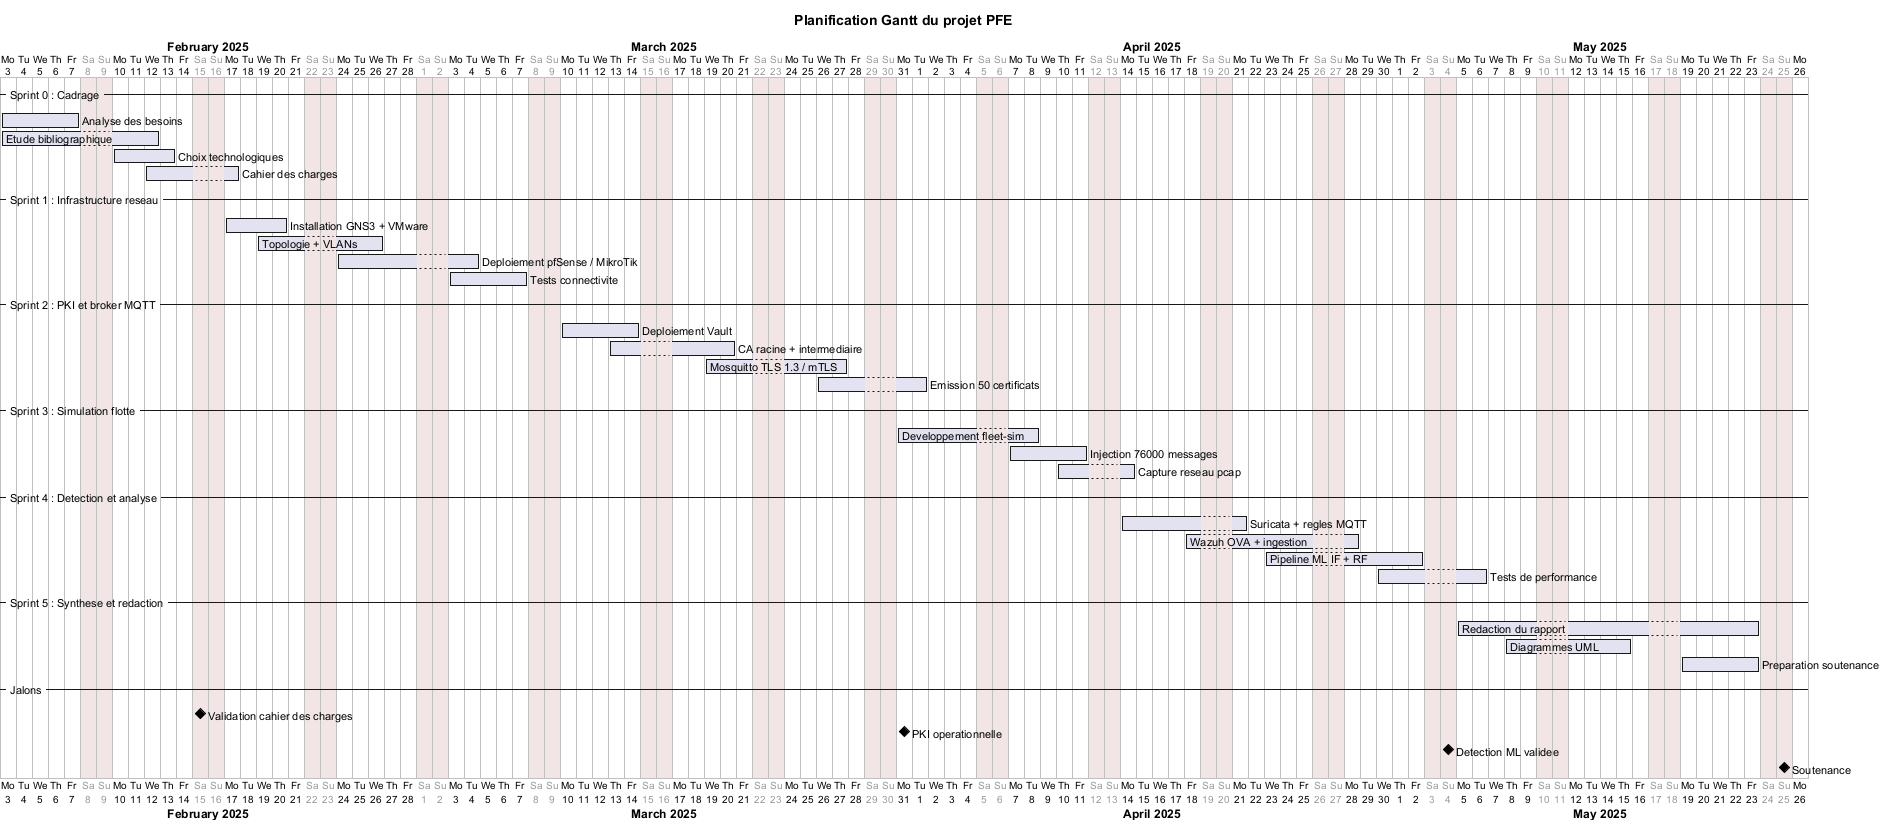
\includegraphics[width=\textwidth]{diagrams/diag-gantt.png}
  \caption{Diagramme de Gantt -- planification du projet PFE}
  \label{fig:gantt}
\end{figure}

La figure~\ref{fig:scrum_sprints} complète cette vision en illustrant le découpage en sprints et la nature des livrables produits à chaque itération.

\begin{figure}[H]
  \centering
  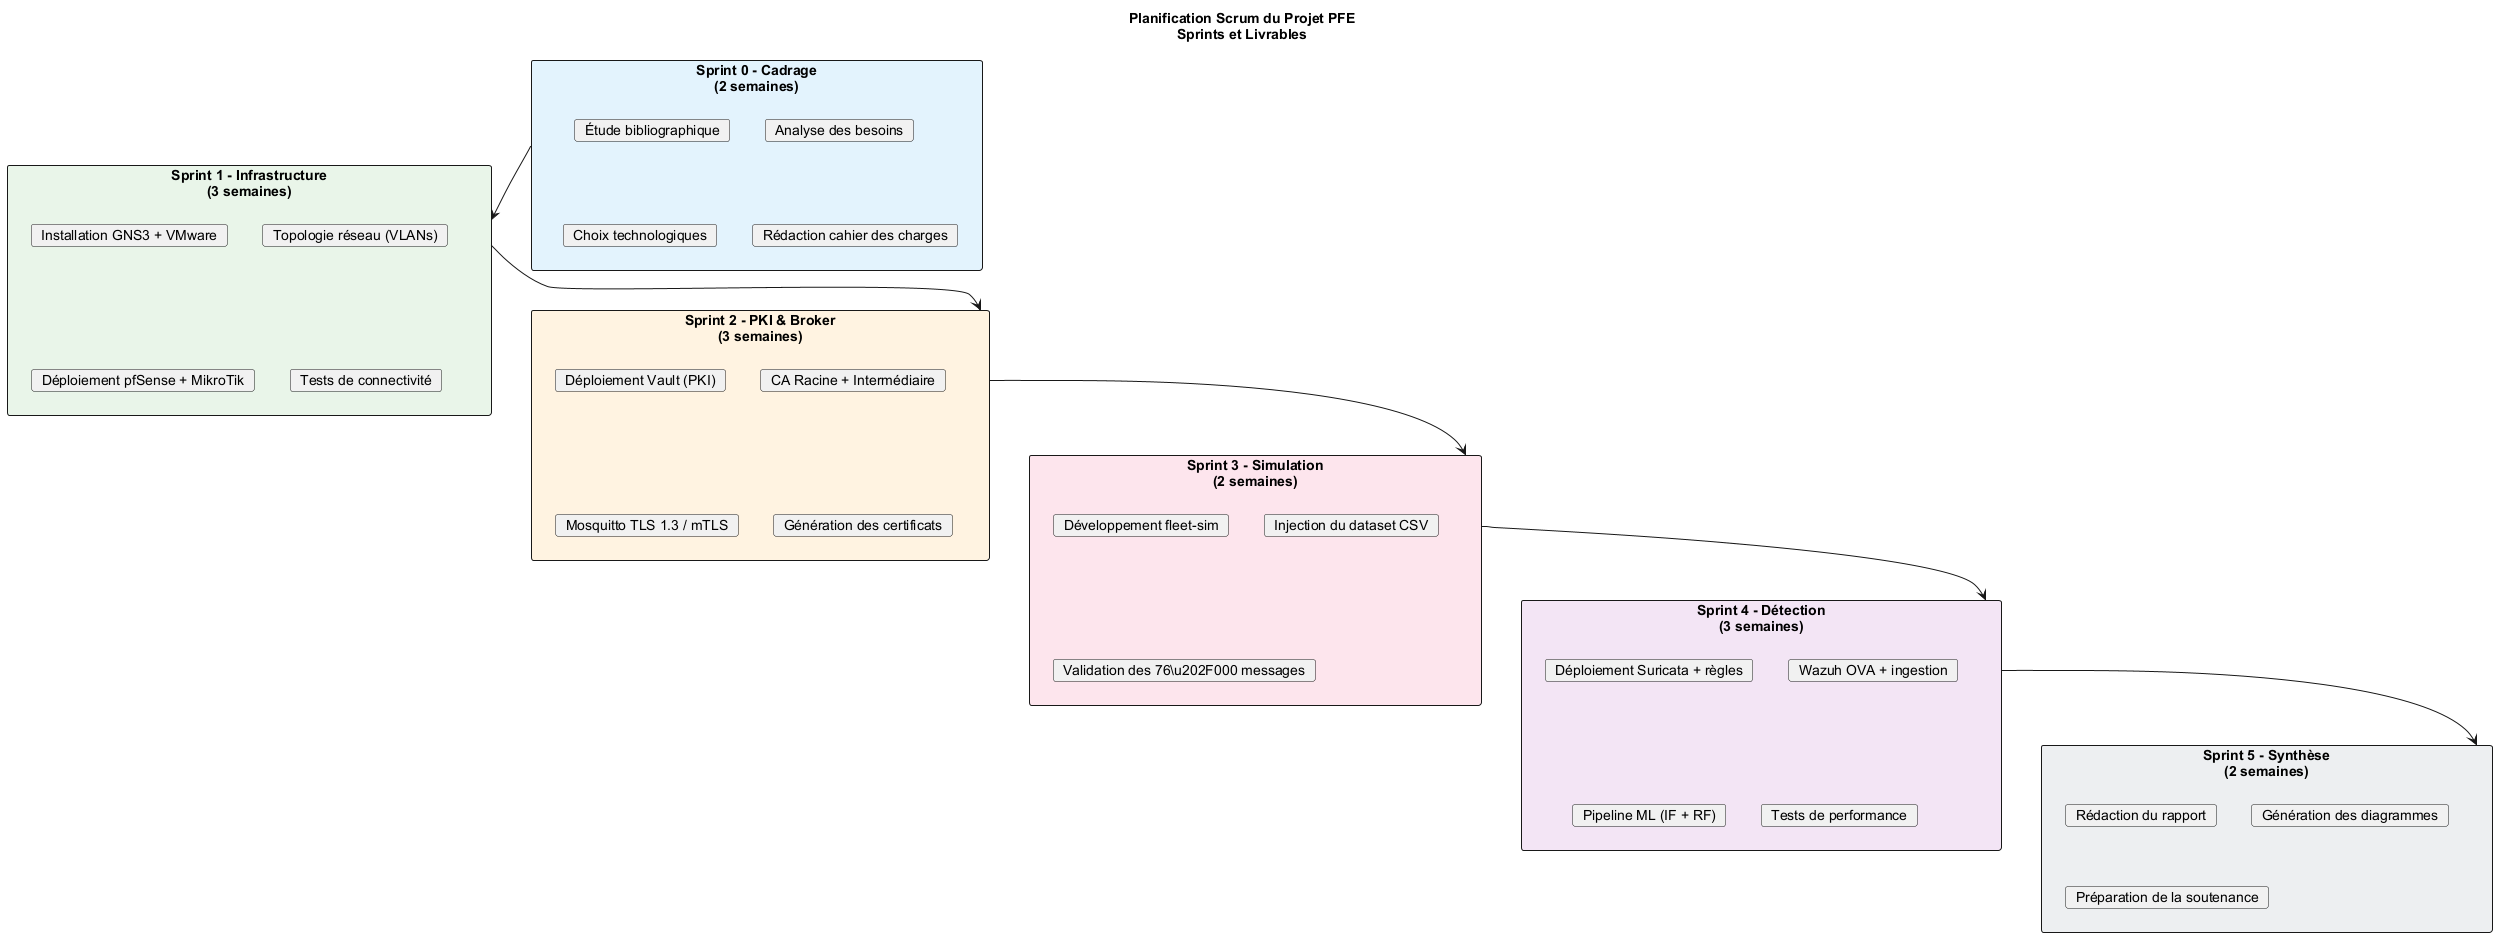
\includegraphics[width=\textwidth]{diagrams/diag-scrum-sprints.png}
  \caption{Planification des sprints du projet PFE}
  \label{fig:scrum_sprints}
\end{figure}

\subsection{Diagramme de cas d'utilisation général}

Pour clore ce cadrage, la figure~\ref{fig:cas_utilisation} présente le diagramme de cas d'utilisation global du système, identifiant les trois acteurs principaux (Dispositif IoT, Administrateur, Analyste SOC) et leurs interactions avec les différents sous-systèmes (PKI, broker MQTT, IDS, SIEM, ML).

\begin{figure}[H]
  \centering
  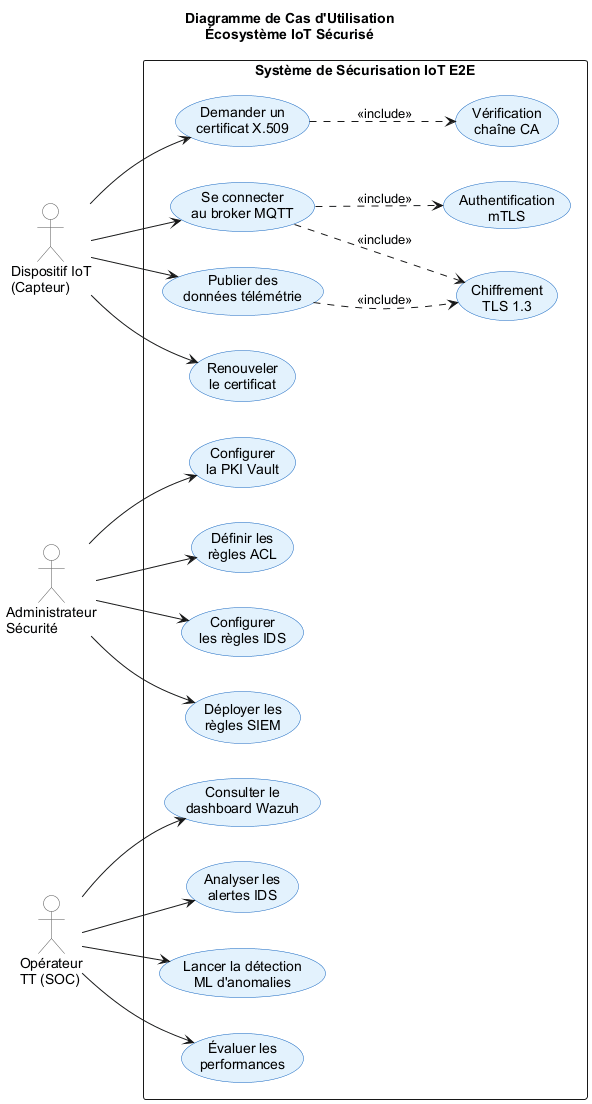
\includegraphics[width=0.85\textwidth]{diagrams/diag-cas-utilisation.png}
  \caption{Diagramme de cas d'utilisation du système IoT sécurisé}
  \label{fig:cas_utilisation}
\end{figure}

\section{Conclusion}

Ce premier chapitre a posé le cadre du projet en présentant \TT{}, son équipe Sécurité des Réseaux, et le contexte stratégique du déploiement d'infrastructures IoT à grande échelle. La problématique de la sécurisation de bout en bout des flux MQTT a été formulée et déclinée en quatre sous-questions directrices, et la méthodologie Scrum retenue a été détaillée avec son Product Backlog, ses six sprints et son ordonnancement Gantt. Le chapitre suivant approfondit l'analyse des besoins et justifie, à travers un état de l'art ciblé, les choix technologiques retenus pour répondre à cette problématique.
